\chapter{Getting Started with EMFText}

	Generating an advanced Eclipse editor for a new language with EMFText just
	requires a few specifications and a generation step. 
	Basically, a language specification for EMFText consists of a language
	metamodel and a concrete syntax specification. Taking these specifications the
	EMFText generator derives an advanced textual editor, that uses likewise generated
	parser and printer to parse language expressions to EMF models or to print EMF models to
	languages expressions respectively. 
	
	\begin{figure}[ht]
	\centering
		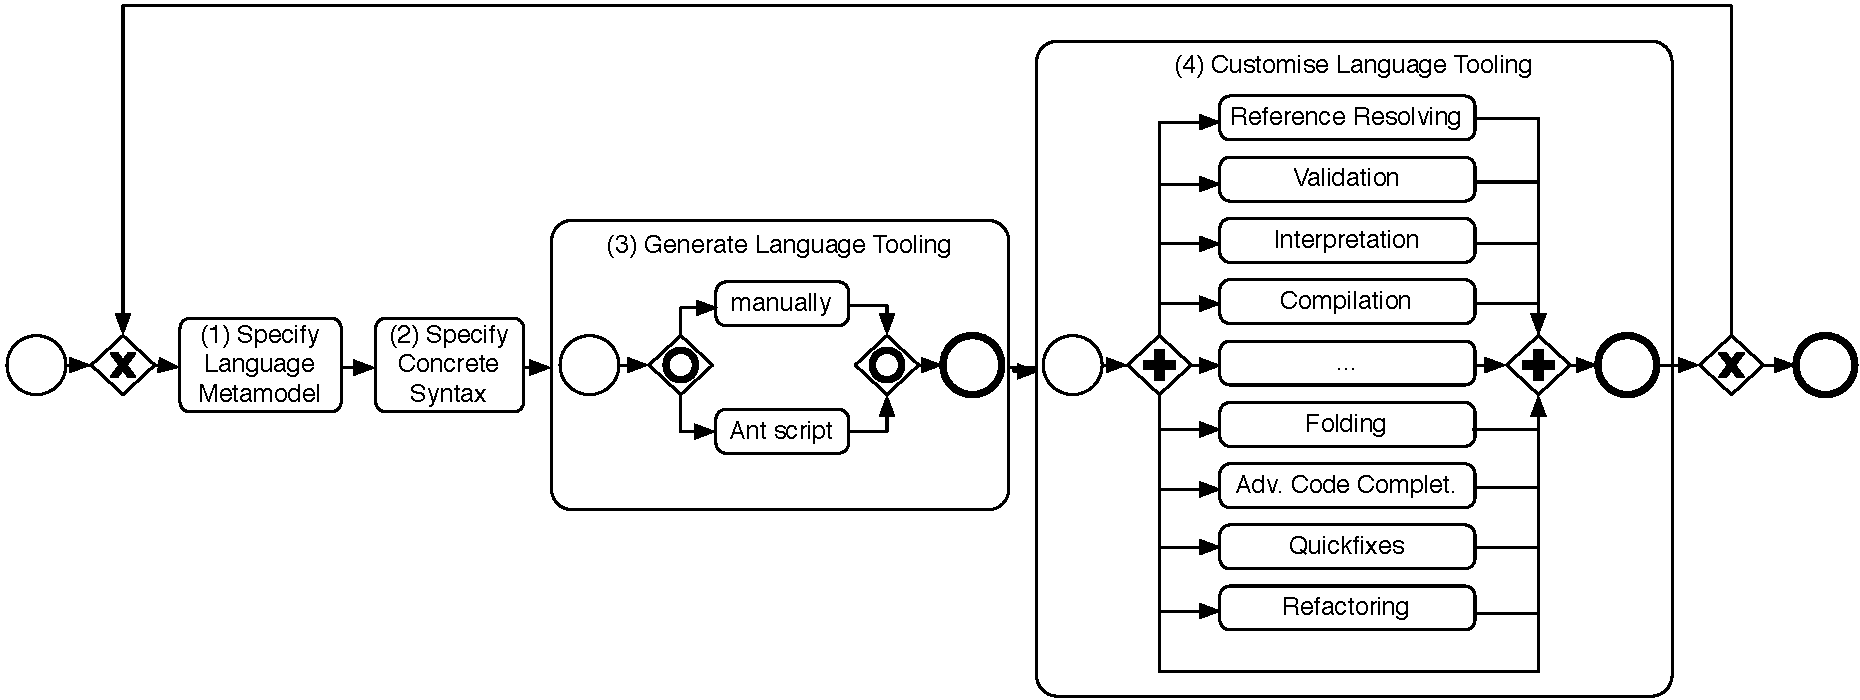
\includegraphics[scale=0.5]{figures/process}
	\caption{Iterative EMFText language development process.}
	\label{fig:process}
	\end{figure}
	
	\noindent The basic language development process with EMFText is depicted in
	Fig. \ref{fig:process}. It is an iterative process that can be passed several
	times and consists of the following basic tasks:
	\begin{description}
	  \item[(1)] Specifying a Language Metamodel,
	  \item[(2)] Specifying the Language's Concrete Syntax,
	  \item[(3)] Generating the Language Tooling,
	  \item[(4)] Optionally Customising the Language Tooling.
	\end{description}
	
	
	
	Each of the these tasks
	will be explained and exemplified in the subsequent sections:
	
	\begin{figure}[ht]
	\centering
		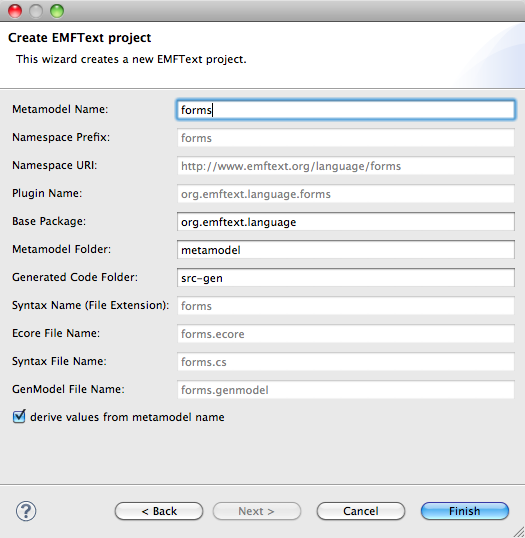
\includegraphics[scale=0.5]{figures/wizard}
	\caption{EMFText Project wizard.}
	\label{fig:wizard}
	\end{figure}

	

	To kick-start the development of a new language you can use the EMFText project
	wizard. Select \emph{File > New > Other... > EMFText Project}. In the Wizard
	(cf. Fig. \ref{fig:wizard}) you just enter the language name and EMFText
	will initialise a new EMFText Project containing a metamodel folder that
	holds an initial metamodel and syntax specification.

\section{Specifying a Language Metamodel}

	As EMFText is tightly integrated with the \EMF language metamodels are
	specified using the Ecore Metamodelling Language. The metamodel specifies the abstract
	syntax of our language. It can be build from \emph{classes} with
	\emph{attributes} that are related using \emph{references}. References are
	further distinguished into \emph{containment} references and
	\emph{non-containment} references. It is important to notice this differences,
	as they have a very different semantics and are also handled differently in
	EMFText. Containment references are used to relate a parent model element and a
	child model element that is declared in the context of the parent element. An
	example which can be found for instance in object-oriented programming
	languages is the declaration of a method within the body of a class declaration. Non-containment
	references are used to relate a model element with an element that is declared
	elsewhere (not as one of its children). An example for programming languages is
	a method call (declared in a statement in the body of a method declaration) that
	relates to the method that it calls using a non-containment reference. The
	referenced method, however, is declared elsewhere: In a class the method
	relates to with a containment reference. 

		\emph{Example.} 
		To define a metamodel for a language, we have to consider the
		concepts this language deals with, how they interrelate and what attributes they
		have. In the following we discuss the concepts of an exemplary language to
		specify forms and how they are represented in a forms metamodel.
		
		\begin{itemize} 
		  \item A Form (class) has a caption (attribute) and contains (containment
		  reference) a number of question Groups (class).
		  \item Each Group has a name (attribute) and contains (containment reference)
		  a number of question Items (class).
		  \item Each Item has a question text (attribute), an explanation
		  (attribute).
		  \item There are various Types of question items (class)  with
		  regard to the answer types they expect: e.g., Text questions
		  (subclass), Date questions  (subclass), Number questions  (subclass),
		  Choices (subclass), or Decisions (subclass).
		  \item Choices and Decisions declare (containment reference) a number of
		  selection Options (class).
		  \item There may be question Items
		  that are dependent of (non-containment reference) the selection of a 
		  particular Option in another Item, 
		  e.g., a question that asks for the age of your children, only if you
		  previously selected that you have some.
		\end{itemize}

	Listing \ref{lst:formsMetamodel} depicts a textual representation of the
	according EMF metamodel. Besides the mapping of forms concepts to Ecore it
	also refines the multiplicities and types. A new text.ecore metamodel is
	created by selecting \emph{File > New > Other... > EMFText .text.ecore
	file}. For a detailed introduction on the basics of Ecore metamodelling we
	refer to \todo{add citation}.

	
	\lstset{language=textecore}
	\begin{lstlisting}[label=lst:formsMetamodel, caption=Metamodel for the
	exemplary forms language written in text.ecore] package forms // this is the
package forms // this is the package name 
        forms // this is the namespace prefix
        "http://org.emftext/language/forms.ecore" // the namespace URI 
	{

	class Form {
		attribute EString caption (0..1);
		containment reference Group groups (1..-1) ;
	}
	
	class Group {
		attribute EString name (1..1);
		containment reference Item items (1..-1);
	}

	class Item {
		attribute EString text (0..1);
		attribute EString explanation (0..1);
		containment reference ItemType itemType (1..1);
		reference Option dependentOf (0..-1);
	}

	abstract class ItemType {}

	class FreeText extends ItemType {}
	class Date extends ItemType {}	
	class Number extends ItemType {}

	class Choice extends ItemType {
		attribute EBoolean multiple (0..1);
		containment reference Option options (1..-1);
	}
	class Decision extends ItemType {
		containment reference Option options (2..2);
	}
		
	class Option {
		 attribute EString id (0..1);
		 attribute EString text (0..1);
	}
}

	\end{lstlisting}
	
Each Ecore metamodel is accompanied by an .genmodel. You can create the
	.genmodel by selecting \emph{File > New > Other... > EMF Generator Model}.
	The generator model is used to configure various options for EMF code
	generation (e.g., the target directory). From the root element of the .genmodel
	you can now start the generation of Java code implementing your metamodel
	specification.

\section{Specifying the Language's Concrete Syntax}
\label{sec:process_specification}

After defining a metamodel, we can start specifying our
\emph{concrete syntax}. The concrete syntax specification specifies 
the textual representation of all metamodel
concepts. For that purpose, EMFText provides the cs-language. 
As a starting point, EMFText provides a syntax generator that can
automatically create a cs specification conforming to HUTN (Human-Useable
Textual Notation)~\cite{HUTN} from the language metamodel. 
To manually specify the concrete syntax create a
new syntax specification by selecting \emph{File > New > Other... > EMFText .cs
file}.

\noindent Listing \ref{lst:formsCs} depicts a syntax specification for the forms
language. It consists of five sections: 
\begin{itemize}
  \item In the first section the language file
	extension is defined, the syntax specification is bound to the metamodel
	Furthermore, and the syntax start symbol defined.
  \item In the second section various EMFText code generation options can be
  	configured.
  \item  In the third section basic token types used by the language
  	lexer to tokenise language expressions are defined. If no token definitions
 	are given, default token types are used. 	
  \item In the fourth section token styles are defined that customise syntax
  	highlighting for specific token types in the generated editor
  \item In the fifth section the syntax rules for the language are specified.	
\end{itemize}

	The syntax specification rules used in the cs-language are derived from the
	EBNF syntax specification language to support arbitrary context-free languages.
	They are meant to define syntax for EMF-based metamodels and, thus, are
	specifically related to the Ecore metamodelling concepts. Therefore, it provides
	Ecore-specific specialisations of classical EBNF constructs like terminals, and
	non terminals.

\todo{sketch the benefit of that specialisation}

	In the following we conclude the most important syntax specification
	constructs found in the cs-language and their relation to EBNF and Ecore
	metamodels. For an extensive overview on the syntax specification language we
	refer to Sect. \ref{chap:cs}.

	\begin{description}
       \item[Rule] An cs rule is a is related (by its name) to a specific
		class from the metamodel. It defines the syntactic representation of this
		metaclass, its attributes and references. All syntax rules are collected in
		the rules section of the cs file. Within syntax rules various constructs like
		keywords, syntax terminals, non-terminals, and EBNF operators as
		multiplicities (?, +, *), alternative (|), or rounded brackets 
		to nest sub-rules can be used.
		
		Examples: \begin{verbatim}Form ::= ...;, Group ::= ...;\end{verbatim}
        
       \item[Keywords] Keywords are purely syntactic elements that are mainly
        used to structure and markup particular language expressions.
        
        Examples: \begin{verbatim}"FORM", "GROUP", "ONLY" "IF" \end{verbatim}
        
        
       \item[Attribute Terminal] Attribute terminals are used in rule bodies to
        specify the syntactic representation for attributes of the according
        meta class. They can be recognised by the attribute name that is followed
        square brackets. Within these square brackets a token that specifies
        the syntax allowed for attribute values, or a prefix and a suffix that
        must surround attribute values can be given. If nothing is given a
        default text token is assumed.

        Examples: \begin{verbatim}name[], mulitple[MULTIPLE], name['"','"']\end{verbatim}


       \item[Containment Reference Non-Terminals] Containment reference non-terminals
       are used in rule bodies to specify the syntactic representation for
       containment references of the according meta class. They use the
       reference name and are not followed by a bracket. They are derived from
       EBNF non-terminals, which means that during parsing the parser descends
       in the syntax rule specified for the class the
       containment reference points to.

       Examples: \begin{verbatim}groups, questions\end{verbatim}

       \item[Non-Containment Reference Terminals] Non-containment reference
       terminals are used in rule bodies to specify the syntactic
       representation for non-containment references of the according meta
       class. They use the reference name that is followed square brackets.
       Within these square brackets an token specifies the syntax allowed for
       expressions in the concrete syntax that identify the element the
       non-containment reference relates to. This symbolic reference is later
       resolved to the actual element (cf.
       Sect.~\ref{sec:cust_reference_resolving}).

       Examples: \begin{verbatim}dependentOf[]\end{verbatim}
       
       \item[Printing Markup] Printing Markup is used to customise the behaviour
       of the generated printer. This is useful to achieve a particular standard
       layout for printed language expressions. Two forms of printing markup are
       supported: 
       \begin{itemize}
         \item whitespace markup, prints a given number of
         whitespaces \texttt{\#<n>}
         \item  and linebreak markup, introduces a linebreak followed by a given 
         number of tab characters \texttt{!<n>}
       \end{itemize}
    \end{description}

 \lstset{language=cs}
	\begin{lstlisting}[label=lst:formsCs, caption=Concrete syntax specification for
	the exemplary forms language written in the cs-language] 
SYNTAXDEF forms
FOR <http://www.emftext.org/language/forms>
START Form

OPTIONS {
	overrideBuilder = "false";
	additionalDependencies = "org.emftext.language.forms.generator";
}

TOKENS {
	DEFINE MULTIPLE $'multiple'|'MULTIPLE'$;
}

TOKENSTYLES {
	"TEXT" COLOR #da0000;
	"FORM" COLOR #000000, BOLD;
	"ITEM" COLOR #000000, BOLD;
	"CHOICE" COLOR #000000, BOLD;
	"ONLY" COLOR #da0000, BOLD;
	"IF" COLOR #da0000, BOLD;
	"DATE" COLOR #000000, BOLD;
	"FREETEXT" COLOR #000000, BOLD;
	"NUMBER" COLOR #000000, BOLD;
	"DECISION" COLOR #000000, BOLD;
	"GROUP" COLOR #000000, BOLD;
}
  
RULES {
	Form ::= "FORM" caption['"','"'] !1 groups*;
	Group ::= !0 "GROUP" name['"','"'] !0 items*;
	Item ::= "ITEM" text['"','"'] ( explanation['"','"'] )? 
				("ONLY" "IF" dependentOf[])? ":" itemType !0;
	Choice ::= "CHOICE" (multiple[MULTIPLE])? 
				"(" options ("," options)* ")";
	Option ::= ( id[] ":")? text['"','"'];
	Date ::= "DATE";
	FreeText ::= "FREETEXT";
	Number ::= "NUMBER";
	Decision ::=  "DECISION" "(" options "," options ")"; 
}

	\end{lstlisting} 
 


\section{Generating the Language Tooling}
\label{sec:process_generating}
	Given a complete syntax specification the EMFText code generator can be used to
	derive an advanced textual editor and a accompanying customisable
	language infrastructure. Basically there are two ways to use the code
	generator: Manually within Eclipse or from an Apache Ant script.


	\subsection{Generating Resource Plug-ins in Eclipse}
	Manual code generation can be triggered form the context menu of the concrete
	syntax specification. Therefore, right click the cs file and select
	\emph{Generate Text Resource}. This starts the EMF code generator that produces
	a number of plug-ins. Fig. \ref{fig:generationResults} depicts the plug-ins
	generated for our exemplary forms language. In the following we shortly discuss
	their purpose:
	
	\begin{itemize} 
	  \item \texttt{org.emftext.commons.antrl3\_2\_0} This projects contributes the
	  ANTLR parsing runtime that the generated parser for the forms language
	  depends on. As EMFText is meant to be runtime free the Antlr runtime is generated
	  for every new language, of no runtime is found in the current workspace.
	  \item \texttt{org.emftext.language.forms} This is the basic plug-in of the
	  language. In the folder \texttt{metamodel} it contains the Ecore metamodel
	  and the cs specification defined previously. The \texttt{src-gen} folder contains the Java-based implementation that was
	  generated using the .genmodel.
	  \item \texttt{org.emftext.language.forms.resources.forms}
	  This is the plug-in that contains the generated parser, printer and various
	  infrastructure for the forms language. The project contains two source
	  folders (\texttt{src} and \texttt{src-gen}). The contents of \texttt{src-gen}
	  is overridden by every run of EMFText code generation. It is, thus not meant
	  to contain manually customised code. The contents of the \texttt{src} folder
	  contains implementation classes that are meant for manual customisation. By
	  default it only contains reference resolvers that are used to resolve
	  symbolic names of non-containment references to the model element actually
	  meant. For details on reference resolving we refer to Sect.
	  \ref{sec:cust_reference_resolving}. Various cs options are available to
	  tailor what language implementation artifacts shall be customised and, therefore, 
	  put into the \texttt{src} folder. For a
	  detailed discussion of such options we refer to Sect. \ref{sec:overriding_generated_classes} and
	  Appendix \ref{app:options}.
	  
	  Besides the files implementing the language tooling, a number of extension
	  points specific for the language are generated to the \texttt{schema} folder. 
	  They can be used to further customise language tooling. For details we refer
	  to Sect. \ref{sec:using_generated_extension_points}.
	  
	  \item \texttt{org.emftext.language.forms.resources.forms.ui} This plug-in 
	  contains all generated classes related to the Eclipse-based User Interface
	  (UI). Such separation of implementation belonging to the UI or not, enables
	  the application of the language backend detached from the Eclipse UI.
	\end{itemize}
	
	\begin{figure}[ht]
	\centering
		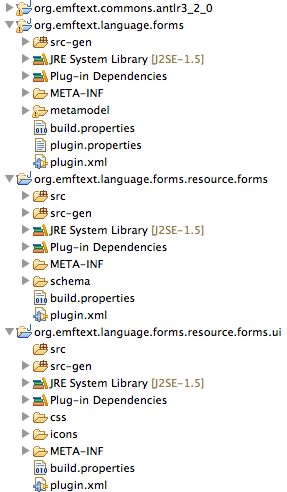
\includegraphics[scale=0.7]{figures/generationResults}
	\caption{Projects generated by EMFText to implement language tooling.}
	\label{fig:wizard}
	\end{figure}

	\subsection{Generating Resource Plug-ins with ANT}
	\label{sec:process_generating_ant}
	A second way of starting the EMFText code generator is using Apache Ant
	scripts. Therefore EMFText contributes a number of tasks for Apache Ant.
	which are automatically registered to the Eclipse platform using the
	naming scheme: \emph{emftext.taskName}. The following task are shipped with
	
	\paragraph*{GenerateTextResource}~This task can be used to generate all
	language implementation plug-ins. The following listing exemplifies the
	application of this task and its obligatory parameters:
\begin{lstlisting}
<emftext.GenerateTextResource
	syntax="pathToCSSpec"
	rootFolder="path/to/project/root"
	syntaxProjectName="nameOfTheGeneratedProject"
/>
\end{lstlisting}
	Further parameters are \texttt{generateANTLRPlugin="[true|false]"}, which
	specifies whether the additional plug-in
	containing the ANTLR parsing runtime should be generated, and
	\texttt{pre\-processor="[qualified class name]"} referring to an implementation
	of the \emph{org.emftext.sdk.\-ant.Syntax\-Processor} interface. 
	\todo{what does this interface?}
	
	\paragraph*{RegisterEcoreResourceFactory}~This task registers an Ecore
	model's resource factory for a certain type. 
	\todo{why may this be required?}
	The following listing exemplifies its application:
\begin{lstlisting}
<emftext.RegisterEcoreResourceFactory
	className="qualified.factory.class.name"
	type="qualified.ecore.type.name"
/>
\end{lstlisting}
	\paragraph*{RegisterURIMapping}~This task adds an URI mapping to the EMF URI
	map. 
		\todo{why may this be required?}
	The following listing exemplifies its application:
\begin{lstlisting}
<emftext.RegisterURIMapping
	from="sourceURI"
	to="targetURI"
/>
\end{lstlisting}

\paragraph*{RemoveURIMapping}~This task removes an URI mapping from the EMF's
URI map. 
	\todo{why may this be required?}
The following listing exemplifies its application: 
\begin{lstlisting}
<emftext.RemoveURIMapping
	from="sourceURI"
/>
\end{lstlisting}
	
	
	To execute Ant script that use EMFText task from within your Eclipse runtime,
	you have to adjust the script's run configuration. Therefore, select 
	\emph{Run > External Tools > External Tools Configurations...} and select the
	your Ant script's run configuration. In the \emph{JRE} tab you have to
	activate the \emph{Run in the same JRE as the workspace} option to make the
	EMFText tasks available to the script.
	
\section{Optionally Customising the Language Tooling}

The previous steps are mandatory to generate an initial implementation of
advanced language tooling for your language. The generated text editor already
comes with a number of advanced editing features that help editing language
expressions a lot. However there are various ways to make your language tooling
more useful. EMFText will helps you in customising your language tooling with a
number of additional functions ranging from semantic validation of language
expressions, language compilation, language interpretation, or editor functions
like folding, custom quickfixes, extended code completion, refactoring and more.
To discover the full spectrum of what is possible please consider Sect.
\ref{chap:customisation}.
